% main.tex — JSys submission (double-blind, problem paper).
% Uses the official JSys template (jsys.sty, plainurl.bst) from
% github.com/jsysresearch/template: 7in x 9in text block, two columns,
% 0.33in gutter, 10pt Times, 12pt leading. Grounded in the project's local
% measurement record; every number carries its condition. No author names,
% affiliations, acknowledgements, or funding.
\documentclass[letterpaper,twocolumn,10pt]{article}
\usepackage{jsys}
\microtypecontext{spacing=nonfrench}
\usepackage{graphicx}
\usepackage{amsmath}
\setlength{\parskip}{0pt}
\renewcommand{\arraystretch}{1.05}
\makeatletter
\setlength{\@fptop}{0pt}
% Override the template's \@maketitle to drop the "Anonymous authors / Paper
% under double-blind review" line; the 2.5in title box keeps layout unchanged.
\def\@maketitle{\newpage
 \vspace*{-1in}
 \vbox to 3.7in{
 \vspace*{\fill}
 \vskip 2em
 \begin{center}%
  {\Large\bf \sc \@title \par}%
  \vskip 1.2em
  {\large\normalfont Yue Zheng\par}%
  \vskip 0.35em
  {\small\normalfont South China Normal University\par}%
  \vskip 0.35em
  {\small\normalfont ORCID 0009-0001-6730-0935\par}%
  \vskip 0.35em
  {\small\normalfont Preprint DOI: \href{https://doi.org/10.5281/zenodo.24456762}{10.5281/zenodo.24456762}\par}%
  \vskip 0.9em
  {\small\itshape\normalfont Author version, released alongside the preprint record; the double-blind version under review carries no author names.\par}%
 \end{center}%
 \par
 \vspace*{\fill}
 }
}
\makeatother

\title{\textbf{Problem: 8\,GiB, 306--330\,GB/s, 50/115\,W: A Measured Boundary Map for Fully Resident LLM Inference}}
\author{Yue Zheng, South China Normal University}
\date{}

\begin{document}
\maketitle

\begin{abstract}
Fully resident LLM inference on 8\,GiB clients is usually reported as engine
deltas, yet on such machines the deltas that matter often belong to the
hardware and the measurement. This paper characterizes one consumer laptop
through three walls---8151\,MiB usable VRAM, 33.7\,GB/s single-channel memory,
and a 50/115\,W envelope---and a measured 306--330\,GB/s device interval that
removes 17\,tok/s of nominal headroom. A 20-model capacity matrix, a
parity-gated prefill study, three speculative attempts, and a decode energy
ledger locate the frontier. Against upstream \texttt{llama.cpp}, plain decode
is within $\pm1.1\%$ on ten distinguishable models; seven are unmeasurable
under 40\% power-state variance. At 520 tokens, decode again differs by 2.7\%,
but prefill does not: the parity-locked default takes 4105\,ms versus 286\,ms
upstream (253\,ms with an explicit 512-row batch), and the MTP path takes
8280\,ms versus 303\,ms. Two traps are
documented: a 91\%$\rightarrow$20.0\% attribution reversal and a batch-width
flip at index 41 on an 8-token prompt. The deliverable is a measurement
protocol and a boundary map.
\end{abstract}

\noindent\textbf{Keywords:} fully resident inference; measurement
methodology; consumer GPUs; speculative decoding; time-to-first-token;
power envelope.
\par\medskip

\section{Introduction}

An 8\,GiB client is a common target for local inference, and comparisons on
such clients are usually published as throughput deltas between engines. The
measurement record of this project shows that this framing hides two failure
modes: nominal specifications create headroom that does not exist, and power
management creates deltas that do not belong to the engine. A third failure
mode is internal to the engine itself: a time ledger whose subtraction rule is
wrong can pass every consistency check and still point optimization in the
wrong direction.

The project behind this paper forked a Windows disk-streaming llama.cpp
derivative into a fully resident engine with a frozen C ABI, then spent its
budget on measurement: a hardware probe before any code, a 20-model capacity
matrix, a same-round paired comparison against upstream \texttt{llama.cpp},
and a sequence of gates that make numerical divergence decidable. Three
observations motivate the problem statement.

First, the device's nominal bandwidth (384--448\,GB/s for 128-bit GDDR7 at
24/28\,Gbps) implies about 67\,tok/s for a 9\,B Q4 model, while the measured
effective interval (306--330\,GB/s) implies about 50\,tok/s. The 17\,tok/s
difference is a specification artifact. For planning purposes the measured
interval, not the datasheet, is the one that binds. Second, on ten models whose clock
state allowed resolution, plain decode differences against upstream fall
within $\pm1.1\%$ (absolute mean 0.67\%, sign inconsistent: eight higher, one
lower, one tied); seven larger models are unmeasurable, because the same model
and engine differ by up to 40\% across rounds as the laptop switches between
50 and 115\,W envelopes. Third, the model's native multi-token head accelerates
decode (54.08 to 75.20\,tok/s in the 520-token round) but keeps prefill
token-by-token for numerical alignment: the fork's speculative path takes
8280\,ms against upstream's 303\,ms on a 520-token prompt, while its
explicit-512 plain path takes 253\,ms against 286\,ms. The penalty belongs to
the fork's cross-path parity contract, not to multi-token prediction.

\textbf{Thesis.} For pure-GPU, fully resident inference on an 8\,GiB client,
the achievable frontier is set by measured effective bandwidth, capacity
arithmetic, and power state. Upstream mechanisms such as chunked prefill and
multi-token prediction help inside that frontier, and their admission is
gated by bitwise parity, because batch width and quantization move logits
enough to flip greedy choices on short prompts.

The constraint minimizes TTFT (time to first token) and maximizes tok/s:
\begin{equation}
\begin{aligned}
\min\ & \mathrm{TTFT},\ \max\ \mathrm{tok/s}\\
\text{s.t.}\ & V \le 8151\ \mathrm{MiB},\quad
B_{\mathrm{eff}} \le 330\ \mathrm{GB/s},\\
& P \in \{50,115\}\ \mathrm{W}.
\end{aligned}
\label{eq:constraint}
\end{equation}

In Equation~\ref{eq:constraint} the power term is a set: switching between the
two envelope states moves throughput more than the engine does.

\textbf{Contributions.}
\begin{itemize}
\item[C1] A screening method built on measured limits: capacity, memory-channel,
and power screening in the order they are hit; a four-layer bandwidth probe; and a
decode roofline built from the measured interval, which exposes the
17\,tok/s nominal artifact and classifies each model's bottleneck (fixed
overhead, kernel utilization, or bandwidth/power).
\item[C2] Parity-gated configuration admission: a two-part gate (multi-round
determinism at every length; cross-batch parity enforced where the benefit is
large), a pre-registered margin oracle with a stop rule, and mutation-verified
gates. Parity is width-dependent: the same 9\,B Q4\_0 weights pass at width 1
and diverge at token 38 of the 64-token plain/MTP (multi-token prediction) gate
at width 2---a
quantization-by-width near-tie, distinct from the short-prompt batch-width
flip at index 41 (Section~\ref{sec:prefill}).
\item[C3] A boundary map: the 20-model capacity--rate--TTFT--energy matrix
with four failure classes (capacity rejection, user stop, policy mismatch,
edge degradation), and an 18-model same-round upstream comparison graded into
10 distinguishable, 7 unmeasurable, and 1 loosely resolved.
\item[C4] Measurement traps as first-class results: the
91\%$\rightarrow$20.0\% attribution reversal, the 40\% power-state confounder,
an environment-variable false positive, and a last-token state trap in prefix
reuse---each with its detection path and correction---plus a research agenda
ordered by milliseconds saved per unit of risk.
\end{itemize}

The sections that follow keep this order. Section~2 fixes the conditions of
measurement, Section~3 measures the walls, Sections~4--6 test prefill, decode,
and speculation against them, Section~7 reconstructs the ledger that first
misread the speculative path, and Sections~8--10 extend the record to twenty
models, to upstream, and to the hardening work that keeps the numbers
trustworthy.

\section{Configuration, Lineage, and Measurement Boundary}

Before any timing, the study had to fix what a measurement may assume: what
stays resident, what the interface guarantees, and where one measurement ends
and the next begins. This section sets those conditions.

\textbf{Pure residency.} All weights remain in device memory during decode;
the configuration removes PCIe and storage from the decode path, at the price
of making capacity, bandwidth, and power simultaneously binding.

\textbf{Lineage.} The direct upstream is a Windows disk-streaming fork of
llama.cpp~\cite{llamacpp,diskinfer} (Apache-2.0 at the forked snapshot), whose
residency hook reads tensors into a fixed arena per graph node at disk
speed---about 1.1\,s per token for a 6\,GB model on the local volume. That hook
has only a CPU implementation and is mutually exclusive with CUDA offload; the
resident engine disables it before the first load. The fork inherits llama.cpp
0.7.0 / ggml 0.27.0 through this lineage---quantization kernels, KV layout,
CUDA graphs, and the speculative loop---while the prebuilt comparison binary is
upstream b12202 (0.9.0-dev, commit \texttt{d6be06557}). The project's own
additions are a thin C ABI layer, a tier-memory slot allocator, and a CUDA
node-residency callback; the fork stays read-only outside those additions, and
every rebase re-runs the gates.

\textbf{The interface as measurement boundary.} The C ABI was frozen before
feature work and grows append-only, so old hosts keep working across versions. One
engine serves one generation at a time and the stats snapshot reports the last
completed request; measurements therefore run single-stream. Cancellation is
session-scoped, separating a reusable cancelled session from an undefined
model/OOM session. Appendix~\ref{app:abi} gives the size, error-code, and
concurrency rules behind these measurements; Appendix~\ref{app:glossary}
defines the recurring terms. Single-stream handling is a deliberate choice
rather than a limitation: it keeps queueing time out of every number that
follows.

With residency fixed and the interface pinned, the next step is to measure the
walls themselves, in the order a model meets them.

\section{Physical Walls and Measured Effective Bandwidth}

A fully resident engine removes PCIe and storage from the steady-state path,
so what remains is physical: capacity, the memory channel, the power envelope,
and the cost of the operations that keep the device busy. This section measures
those limits before any engine comparison is attempted.

\textbf{Three walls, in screening order.} Capacity first. Usable VRAM is
8151\,MiB, not the nominal 8192, and a desktop baseline of about 1.1\,GiB (idle
samples 1100--1190\,MiB at 17.8--19.8\,W) is subtracted before any model
arithmetic.

\textbf{Memory.} One DDR5-5600 stick sustains 33.7\,GB/s at 16 threads; a
CPU-only fallback runs at 6.0\,tok/s for the 9\,B model (167\,ms/token),
12.5\,tok/s for 4\,B, and 6.7\,tok/s for 8\,B---two orders of magnitude below
the resident path.

\textbf{Power.} The 9\,B Q5 model at \texttt{-p512 -n128 -r10} averages
104.65\,W over the active segment, peaks at 109.28\,W, averages 70\,$^\circ$C
and peaks at 74\,$^\circ$C, with SM at 2713.9\,MHz and 93.3\% utilization. The
device ceiling is 115\,W; at 74\,$^\circ$C there is no thermal throttling.
Temperature has headroom; power does not.

\textbf{Device (Table~\ref{tab:bw}, Figure~\ref{fig:bw}).} Device memory
measures 306.3\,GB/s copy read--write, 329.7\,GB/s on a pure-read kernel, and
307.6\,GB/s device-to-device. The study uses 330 for the decode
roofline~\cite{williams2009} (weights read once per token) and 306 for
cross-layer ratios (mixed read/write); mixing the two shifts the roofline by
7\%. That 7\% is the width of the band in which a nominal reading can hide a
real shortfall: a model planned against 329.7\,GB/s is planned against a
number the hardware does not sustain for mixed traffic.

\textbf{Host.} Host interconnect is size-dependent (Table~\ref{tab:bw}).
Pinned transfers reach 26.66/27.08\,GB/s at 256\,MiB warm, while a cold first
transfer pays a 2.2$\times$ warm-up penalty and 4\,KiB pages collapse to
0.37\,GB/s. Registering existing pages yields 15.2\,GB/s versus 3.5--3.9\,GB/s
for fresh pinned allocation, so buffers are allocated once at startup. An
independent negative sample (a downstream fork's per-layer pinning at about
0.7\,GB/s) confirms that hot-path pinning is a wall of its own.\footnote{%
Intermediate points, all in Table~\ref{tab:bw}: 23.11\,GB/s at 1\,MiB,
8.28\,GB/s pageable at 512\,MiB, 12\,GB/s cold first; each 4\,KiB transfer
costs 10--14\,$\mu$s.} The lesson for the design is that transfer size, not
link width alone, decides whether a transfer sits on the critical path.

\textbf{Storage.} The local NVMe volume measures 5.10\,GB/s direct I/O versus
3.13\,GB/s buffered on a 4\,GiB sequential read (the working set exceeds the
page cache), 5.56/4.33\,GB/s for 4\,MB sequential/random, and 44.8\,MB/s for
4\,KB random (10{,}943 IOPS, 91\,$\mu$s). Megabyte-aligned blocks are the
natural streaming unit: at 4\,KB the device spends most of its time waiting,
and at 1\,MB and above it approaches the link limit.

\textbf{Kernel.} An empty kernel launch costs 7.51--8.15\,$\mu$s; at about 300
launches per token that is 2.3\,ms, 16\% of a 14\,ms/token budget. Fixed costs
of this size are exactly what a wider batch buys back, which is the subject of
the next section.

\begin{table}[t]
\centering
\small
\setlength{\tabcolsep}{3pt}
\begin{tabular}{@{}>{\footnotesize}l>{\footnotesize}l>{\footnotesize}l@{}}
\toprule
Layer & Measured & Condition \\
\midrule
HBM copy (R+W) & 306.3 GB/s & 1 GiB copy kernel \\
HBM pure read & 329.7 GB/s & 1 GiB read kernel \\
HBM D2D & 307.6 GB/s & 1 GiB cudaMemcpy \\
PCIe pinned H2D/D2H & 26.66 / 27.08 GB/s & 256 MiB, warm \\
PCIe pageable H2D & 8.28 GB/s & 512 MiB \\
PCIe cold first & 12 GB/s & first 512 MiB after idle \\
PCIe 4 KiB / 1 MiB & 0.37 / 23.11 GB/s & latency-dominated / ramp \\
Host register / alloc & 15.2 / 3.5--3.9 GB/s & 512 MiB \\
CPU memory & 33.7 GB/s & 16 threads, R+W \\
NVMe direct / buffered & 5.10 / 3.13 GB/s & 4 GiB sequential \\
Volume 4 MB seq / rand & 5.56 / 4.33 GB/s & QD1, unbuffered \\
Volume 4 KB random & 44.8 MB/s & 10{,}943 IOPS, 91 $\mu$s \\
Empty kernel launch & 7.51--8.15 $\mu$s & 10{,}000 launches \\
\bottomrule
\end{tabular}
\caption{Measured bandwidth and latency layers. The roofline uses the
measured interval; the nominal device peak (384--448\,GB/s) appears only in
Figure~\ref{fig:bw} to expose the 17\,tok/s artifact.}
\label{tab:bw}
\end{table}

\textbf{The 17\,tok/s artifact.} At 448\,GB/s nominal, the 9\,B per-token read
implies about 67\,tok/s; at 330\,GB/s measured, about 50\,tok/s. The plain
path's 46.4\,tok/s at default 4k context folds back to about 308\,GB/s
(6.18\,GiB $\div$ 21.55\,ms), inside the measured interval. The native
multi-token path sustains 1.882 tokens per 26.5\,ms step, about 250\,GB/s.
Both are bounded by the measured wall. The roofline serves as an alarm.
Across the 20-model matrix, folded effective bandwidth spans
34.6--321.6\,GB/s and no plain row exceeds 330. A number above 330 indicates a
measurement error (missing weight bytes, an 8-token short run, or a
speculative rate mislabeled as plain). The first knob the study tested against
these walls was prefill scheduling, where one batch-width choice moved TTFT by
an order of magnitude.

\begin{figure}[t]
\centering
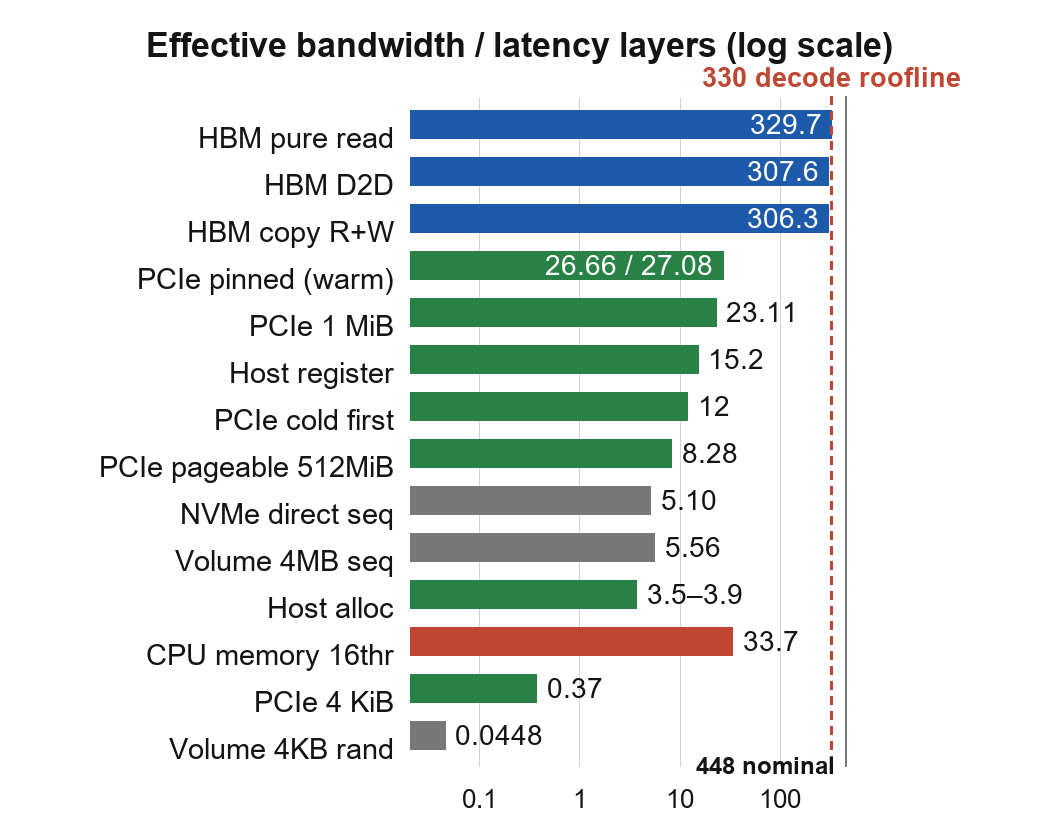
\includegraphics[width=0.98\columnwidth]{fig_bw.png}
\caption{Effective bandwidth layers on the target client (log scale), from
the probe record. The dashed line is the 330\,GB/s decode roofline; the
nominal 448\,GB/s peak exposes the 17\,tok/s artifact.}
\label{fig:bw}
\end{figure}

\section{Prefill: Batch Size as a Numerical Decision}
\label{sec:prefill}

Prefill decides how long a request waits before decode begins, and it is easy
to assume that the cost is set by the model. The record shows otherwise: the
dominant term was a numerical decision about batch width.

\textbf{The nine-second silence.} The first generation path treated each
prompt token as an independent decode call: a 521-token prompt took
9260.4\,ms to first token, with no callback in between---indistinguishable
from a hang. The fix was scheduling: fill one batch. Chunked prefill is the
serving-side form of the same idea~\cite{sarathi2024}: prompt work is split
into bounded pieces so other work can proceed; with one resident request, the
same mechanism appears as a batch-width choice. At batch 2, TTFT fell to
4851.9\,ms (1.91$\times$, the theoretical ceiling for 2 rows); 131-token and
5-token prompts moved 2370.0$\rightarrow$1252.9\,ms and
107.6$\rightarrow$79.6\,ms. The gain shrinks as prompts shorten, because short
prefill was never the dominant cost.

\textbf{An arbitrary cap, and a failure case that exposed it.} The
escape-hatch environment variable was initially clamped to $[1,8]$ with no
measurement behind the 8, while the context's own \texttt{n\_ubatch} is 512. A
deliberate failure run (1\,B, 522 tokens, requested batch 512 against the old
cap) returned \texttt{gain=1.00x} with parity OK, showing the batch never took
effect. After raising the cap to 512 with defaults untouched, TTFT fell
1206.8$\rightarrow$41.2\,ms (29.32$\times$) on 1\,B and
9112.8$\rightarrow$266.7\,ms (34.17$\times$) on 9\,B. Only then were defaults
raised, per architecture, after each candidate passed a 520-token consistency
run: \texttt{llama}, \texttt{qwen3}, \texttt{qwen35}, \texttt{nemotron\_h} get
512; unknown architectures fall back to 1. With defaults in place, four models
at 521--522 tokens gained 29.36/31.11/30.21/31.75$\times$
(1\,B/4.2\,B/Nemotron/8\,B); the 9\,B nextn (native MTP) model, defaulting to
batch 2, gained
1.91$\times$. A profile ratio of 0.99--1.02 confirmed the
default path reaches the intended batch. The four gains cluster because
token-by-token prefill pays a model-size-independent fixed cost (launch,
graph reuse check, batch fill, sampler prep) 521 times instead of twice.

\textbf{The regression that set the nextn default.} Raising the plain default
to 512 broke plain/MTP parity at token 2 (\texttt{plain=1061 mtp=198}): the
speculative path prefills token-by-token on purpose, so both paths must start
from identical numerics. Batch 2 restores 64/64 parity, because 1--2 rows are
bitwise identical to token-by-token while 3+ rows switch the hybrid
state-space model (SSM)
to a chunked delta-net kernel whose accumulation order shifts logits by about
0.13. Models with a native nextn head therefore default to 2---the maximum on
the consistency boundary---and the 9\,B's explicit-512 result
(9178.5$\rightarrow$266.0\,ms, 34.51$\times$) remains available behind the
gate. The same model's two paths have mutually exclusive optima. Three
divergence indices recur in this paper and name different gates: token 2 here
(plain default 512 against token-by-token MTP on the hybrid SSM model), token 38
in the 64-token plain/MTP gate for Q4\_0 at width 2 (Section~\ref{sec:spec}),
and index 41 in the short-prompt batch-width margin oracle below.

\textbf{Two gates.} Short prompts show real cross-shape flips (1\,B at 6
tokens: 1.28$\times$ gain but parity fail; 8\,B at 5 tokens: 2.25$\times$,
fail; Nemotron at 6 tokens: 2.93$\times$, pass), so the gate splits:
multi-round determinism at every length, and cross-batch parity enforced at
the $\approx$520-token tier where the 29--34$\times$ benefit outweighs the
fixed ulp risk. At short lengths cross-batch parity is diagnostic.

\textbf{A margin oracle with a pre-registered stop rule.} The 0.13 shift says
how large the perturbation is, not how much headroom real prompts have. A
diagnostic (env-gated, zero work when off) prints the top1--top2 logit margin
per greedy step on the plain path. The criterion was fixed in advance: minimum
margin at least 0.26 (twice the perturbation), and every true flip's margin
below 0.13; true flips are located by differencing top-1 id sequences across
runs (4 candidates, 1 true flip in the short run). Results: the 8-token
default prompt has minimum margin 0.0549 (0.42$\times$) at narrow batch and
0.0080 (0.06$\times$) at 512; the first divergence is at index 41 (id 58737 vs
9357), after which 86 of 128 ids differ---one flip, then path separation. The
521-token prompt has margins 1.4155 (10.89$\times$) and 1.5411
(11.85$\times$), zero flips, while 127 of 128 margins differ from the fourth
decimal---batch width moves numerics without moving decisions---and TTFT falls
4224.97$\rightarrow$252.49\,ms (16.7$\times$). The pre-registered rule failed
on the short tier; production defaults stayed unchanged while the long tier
gained 16.7$\times$. Index 41 became a permanent regression point.

\textbf{A false positive that became methodology.} The first wide-batch short
run was bitwise identical to narrow batch---margins unchanged to the last
digit, while the long-prompt run had shown fourth-decimal movement. The
environment variable never entered the process. The corrected protocol
requires an in-band witness that the variable took effect (margins must move)
before any conclusion is drawn. The same discipline caught the arbitrary-cap
failure above.

\textbf{Mutation evidence defines what each gate guards.} Mutating the default
batch back to 1 while keeping the old assertions left the gate green
(\texttt{profile=1.91} inside the 0.5--2.0 window). A nearest-neighbor
criterion
($|\mathrm{def}-\mathrm{expected}| < 0.5\,|\mathrm{def}-\mathrm{sequential}|$)
turns the same mutation red (\texttt{def\_err=4507.2}, \texttt{seq\_err=1.9},
\texttt{match=FAIL}; a repeat gave 4156.4---different magnitude, same verdict).

\textbf{Prefix reuse: a probe that demoted a branch.} Prefix reuse is the
serving-side counterpart of this saving~\cite{promptcache2024}. Re-prefilling
the whole history each turn re-pays the cost above. A standalone two-round probe crashed
four times with CUDA illegal access; the crash traced to probe context
parameters that did not reproduce the engine's (q4 KV, rollback slots, graph
capture), so the probe moved inside the engine behind an env-gated two-round
mode and passed first try: an agent prompt (163+64 tokens, second turn 243,
common prefix 227) reused at 131.13\,ms versus 1951.45\,ms fresh
(14.88$\times$) with 0/64 divergence; a short prompt (29+8$\rightarrow$41,
common 37) at 38.76 vs 315.50\,ms (8.14$\times$), 0/8. The shared-prefix delta
was exactly 0 in both: the assumed BPE re-tokenization mismatch at the splice
never occurred, so the planned bounded-trimming branch was demoted to an
unexercised fallback. Two traps were recorded: at batch 512 the fresh side is itself a
different numerical trajectory, so 41/64 differences there measure
cross-batch comparison---bitwise claims compare against the engine-default
fresh run; and the sampling loop delivers the last token without decoding it,
leaving state one row short (54/64 divergence in a field note), fixed by
decoding the final row before continuation. The probe covers two rounds on
one model's plain path. With prefill bounded, the next question is what decode
can reach at all.

\section{Decode Ceiling and Energy: Three Different Bottlenecks}

Decode is the steady state that dominates a long generation, so it is where a
ceiling matters most. This section recalibrates that ceiling on one build and
one machine state, then asks what each model is actually limited by.

Before optimizing, the study recalibrated its own ceilings: earlier numbers
(4\,B about 92, 8\,B about 64, 1\,B about 336) came from mixed rounds, mixed
memory clocks, and 8-token runs. The recalibration fixed one build, one round,
one machine state; 317--329-token prompts; 64--128 generated tokens; q4 KV;
one warmup plus three timed runs; and per-token time split into eval, sampler,
detokenize, callback, and host gap.

\begin{table}[t]
\centering
\small
\setlength{\tabcolsep}{3pt}
\begin{tabular}{@{}lrrrr@{}}
\toprule
Model & tok/s & eval ms/tok & eff.\ GB/s & roofline \\
\midrule
MiniCPM5 1B & 308.3 & 3.02 & 226 & 73\% \\
qwen3.5 4.2B & 81.8--85.9 & 11.70 & 231 & 74\% \\
Nemotron 4B & 95.1--96.7 & 10.10 & 281 & 85\% \\
DSR1 8B & 57.1 & 17.21 & 292 & 97\% \\
\bottomrule
\end{tabular}
\caption{Ceiling calibration, same round (317--329 prompt tokens, 64--128
generated, q4 KV). Effective bandwidth = weight bytes $\div$ eval time.
Roofline includes KV and recurrent state where applicable.}
\label{tab:ceiling}
\end{table}

Two suspects were eliminated first: CUDA graph rebuild counts were zero
(reuse grew from 219 to 4359), and host fixed costs (detokenize
0.002--0.003\,ms, callback $<$0.001, sampler 0.09--0.19, host gap
0.15--0.37\,ms/token) sum to 2.5--4.6\% for 4\,B/8\,B and 7.2\% for 1\,B.
Zeroing the host side still leaves 4\,B near 85\,tok/s. The remaining gaps
have different causes (Table~\ref{tab:ceiling}): the hybrid-SSM 4\,B model
reads at 231\,GB/s (74\% of the roof) because its recurrent segments do not
fill large matmuls---a kernel-utilization problem, confirmed by the same-size
Nemotron reaching 85\%; the 8\,B model reads at 292\,GB/s (97\%) but its memory
clock falls 12001$\rightarrow$11001\,MHz ($-8.3\%$) under sustained load at
about 107\,W---a power/clock wall. The 100\,tok/s question is arithmetic: at
330\,GB/s it requires $\le$3.06\,GB/token, while the Q4 8\,B file is 5.03\,GB,
64\% over budget. Context length costs 5--8\% (79.7\,tok/s at 2248 tokens,
75.4 at 8668), from attention and KV reads; q4 versus q8 KV is within noise
(82.1 vs 81.8--85.9)~\cite{kivi2024}, so q4 is chosen to save the
72--144\,MiB that decide whether MTP fits.

\textbf{Energy is the same story in another denominator.} Decode-level
sampling (200\,ms, samples below 20\,W discarded) gives 4\,B: 79.3\,tok/s at
85.3\,W, 1.08\,J/token (0.93\,tok/J, 48 samples); 8\,B: 54.9\,tok/s at
95.8\,W, 1.74\,J/token (0.57\,tok/J, 98 samples). Energy per token rises
1.61$\times$ while weight bytes rise 1.86$\times$: the 8\,B reads nearly full
bandwidth, the 4\,B wastes a quarter of each read, and the energy denominator
amplifies that structural waste. The gap between 1.61$\times$ and
1.86$\times$ is the measure of that waste: the larger model pays less energy
per byte than the smaller one, because its reads keep the bus busy. Across the matrix the spread is 83$\times$
(0.0910\,J/token, 10.986\,tok/J for the 1\,B model; 7.5516\,J/token,
0.132\,tok/J for the edge-degraded 12\,B, whose 46.42\,W average looks frugal
until time is counted). No model in the matrix crosses the 105--109\,W wall;
the binding constraint is time. Process-level energy (2.36/5.33\,J/token)
includes load and prefill and is reported separately. Arithmetic intensity is
about 3.1\,FLOP/B for the 4\,B model, placing the workload in the memory-bound
regime. Speculation is the remaining lever that changes tokens per read rather
than bytes per read, and it is the subject of the next section.

\section{Speculative Decoding: Three Attempts, One Winner, a Width-Dependent Boundary}
\label{sec:spec}

The three attempts below share one test: does the saved target read exceed the
added draft work and the parity cost it imposes? Each attempt answers that
question in a different place.

Speculative decoding is the lever that speeds decode without changing weight
bytes: one read amortized over several tokens~\cite{leviathan2023,chen2023spec}.
Width 1 amortizes to
3.53\,GB/token (about 253\,GB/s, 77\% of the roof), width 2 to 2.80\,GB/token
(about 236\,GB/s, 72\%): throughput up 17\% at 7\% lower bandwidth use. The
remaining headroom sits in verify-step fixed cost.

\textbf{Attempt 1: ngram self-speculation.} The first attempt borrows from
within the prompt itself. A configuration trap came first
(\texttt{size\_n=12, size\_m=1} proposes nothing, because the copyable length
is min(proposal cap, remaining) and always below the minimum); the correct
hybrid-model setting is 1/1. On repetitive text: 144.3\,tok/s, acceptance
1.000, mean length 2.000---+70\% over the same round's plain 82--86, direct
evidence of one read serving two tokens. On natural English: 78.9--80.8\,tok/s,
acceptance 0.474, mean length 1.267; the 2-row verify step grows
12.3$\rightarrow$16.1\,ms (+31\%) while tokens grow only 26.7\%: net $-3\%$.
One switch, +70\% versus $-3\%$, entirely hit-rate dependent. Default off; the
mode targets repetitive/template output.

\textbf{Attempt 2: external draft model.} The second attempt replaces the
guesser with a smaller model. Vocabulary compatibility screens
first (0.6\,B draft shares 0 entries with the 4.2\,B target; same-family
0.8\,B shares all). With the 0.8\,B draft fully on GPU (497.40\,MiB),
acceptance is a healthy 0.829 (mean length 1.829) yet throughput falls
90.5$\rightarrow$61.8\,tok/s: the step grows 10.9$\rightarrow$29.6\,ms because
the small draft is itself dominated by launch/graph/sync fixed costs and needs
2.7--5.3\,s of prefill on a 322-token prompt. Admission turns on cost
structure: draft forward must be far cheaper than one target step. On an 8\,B
target the same arithmetic yields about 50\,tok/s, below plain 57. Rejected.

\textbf{Attempt 3: the model's native multi-token head.} The third attempt
asks the model to propose from its own head, which removes the separate draft
but adds a parity constraint. Multi-head variants
generalize the draft-verify loop~\cite{medusa2024}. The head here is the
multi-token prediction objective introduced for
DeepSeek-V3~\cite{deepseekv3}; upstream llama.cpp merged native draft-mtp
support in 2026~\cite{llamacppmtp}. The measurements below establish its
width-dependent parity boundary and its prefill cost. The 9\,B model was
re-quantized to Q4\_K\_M (5501.86\,MiB, 5.02 BPW) preserving the nextn tensors.
Width sweep: width 1 = 75.43\,tok/s (best 76.42), acceptance 0.855, mean
length 1.855; width 2 = 84.24 (85.50), acceptance 0.685, mean length 2.370;
width 3 = 76.94, acceptance 0.574, mean length 2.723. The peak at width 2 is a
crossing of two slopes: +28\% accepted length against a 2$\rightarrow$3-row
verify cost; at width 3 the 4-row verify catches up. The 100\,tok/s gap is
millisecond-accountable: 128 tokens at width 2 take 54 steps of 27.7\,ms;
100\,tok/s at mean length 2.370 requires $\le$23.7\,ms; Q4 weight reads account
for 16.7\,ms, the remaining about 11\,ms for 3-row verify compute, head
forward, and accept/rollback. It is a kernel-engineering target.

\textbf{Parity carries its width.} Q4\_0 at width 2 averages a usable-looking
79.85\,tok/s, but it diverges at token 38 of the 64-token plain/MTP gate (357
vs 1690). The divergence is a quantization-by-width near-tie, not the
batch-width oracle of Section~\ref{sec:prefill}. Q4\_K\_M and Q5\_K\_M pass at
all widths tested. In the 20-model matrix, run at
default width 1, all three nextn models pass 64/64 (77.3/77.2/75.8\,tok/s).
Q4\_0 therefore passes at width 1 and fails at token 38 at width 2, which is
why every parity statement in this paper carries its width. Default remains
width 1 (higher
acceptance, shorter accepted runs, steadier parity); width 2 is opt-in behind
its own 64-token gate.

\textbf{Rollback slots serve correctness.} The hybrid model trims rejected
drafts from recurrent state via \texttt{n\_rs\_seq} slots (50.25\,MiB each).
Giving the draft context its own slots to enable trimming instead of
checkpoint replay dropped width 2 from 84.2 to 80.3\,tok/s and was reverted.
With the speculative path bounded, the next question is where its time
actually goes, and answering it required a ledger rather than a stopwatch.

\section{The Attribution Ledger and Its Reversal}

The speedups in Section~6 were measured against a path whose own timing was
not yet trustworthy. This section reconstructs the ledger, shows how it first
misread the speculative path, and states what the correction changes.

The speculative path could report 78.19\,tok/s but not where time went. Nine
perf fields (eval, prompt-eval, sampler, step wall-clock, detokenize, callback,
and three graph counters) were zero on that path. They were filled as an
append-only struct extension under a measure-only rule with a three-condition
gate: step wall-clock within 5\% of decode total, eval $>$ 0, and a
non-negative host residual.

Two mutations proved the telemetry read-only. Zeroing all nine fields turned
the gate red while the token stream stayed bitwise identical and throughput
moved only within run-to-run noise (77.80 vs 78.19\,tok/s). Swapping step and
callback prints made both 19\,$\mu$s and also turned the gate red. Binaries
were restored by sha256 and re-verified.

\textbf{The wrong number that passed every check.} Subtracting eval, sampler,
detokenize, and callback from a 128-token request's 1665.381\,ms left
1519.3\,ms---91\% ``host overhead.'' The number was written into two documents
with a plausible explanation, and it was self-consistent: the formula was
pre-written, the residual non-negative, and the gate green.

Three commonsense signals broke it. The first is mechanistic: a loop that only
detokenizes and calls back contains no operation that could consume
11.9\,ms/token, so the number had no path through the code. The second is
comparative: models from the same tree, running under the same host code,
showed 0.87--0.89\,ms, 13$\times$ less, and host overhead should not scale
with the size of the target. The third is a control: the plain path runs the
identical host loop and showed a tiny residual, which places the excess on the
speculative path's accounting rather than on the host. Each signal on its own
is enough to doubt the number; together they point at the ledger. The 91\% was
the sum of two ledger defects, not a property of the engine.

\textbf{Defect one: a missing term.} The verify batch books its time in
\texttt{prompt\_eval\_ms}, which receives any batch with $>$1 queued row. On
the speculative path the entire verify decode therefore lives there, while
\texttt{eval\_ms} holds only the prefill tail---semantics opposite to the
plain path. Subtracting the missing 1314.48\,ms moved the residual to
204.8\,ms (12.3\%).

\textbf{Defect two: prefill statistics leaking past the reset line.} The
remaining 123.93\,ms of ``eval'' sat on a path that should have no single-row
batches. Unsynchronized eval timing accumulates into the next call, as an
upstream FIXME documents, so prefill statistics crossed the request boundary.
The fix pins the boundary: \texttt{llama\_synchronize} then
\texttt{llama\_perf\_context\_reset} after prefill, on both paths.

\textbf{The clean ledger.} Table~\ref{tab:attr} and Figure~\ref{fig:attr} show
the corrected split, and it is symmetric: plain's prompt-eval is zero,
speculative's eval is zero. Each path's zero column is the correctness check.
Host share is 1.9\% plain and 20.0\% speculative (317.3\,ms over 128 tokens,
about 2.5\,ms/token).

\textbf{What the reversal leaves.} Host overhead is real and worth optimizing,
but it is third in line after step count and prefill parallelism: 128 tokens
took 67 verify steps of 1246.95\,ms total. The old ``eval $>$ 0'' criterion,
written under the wrong semantics, would now reject correct runs; it was
rewritten with the ledger. The 91\% figure remains in the record with a
correction block. A non-negative residual is only a lower bound, because a
large missing term makes it easier to pass. The ledger's symmetry is the
stronger check, and the sequence---plausible formula, green gate, wrong
number---is the paper's clearest measurement trap. With the ledger corrected,
the study could compare engines on numbers it could defend, first across
twenty models and then against upstream.

\begin{table}[t]
\centering
\small
\setlength{\tabcolsep}{2.2pt}
\begin{tabular}{@{}lrrrrrr@{}}
\toprule
Path & total & eval & p\_eval & samp & detok+cb & host \\
\midrule
plain & 2304.08 & 2234.53 & 0 & 25.51 & 0.63 & 43.4 (1.9\%) \\
MTP & 1586.24 & 0 & 1246.95 & 21.67 & 0.33 & 317.3 (20.0\%) \\
\bottomrule
\end{tabular}
\caption{Corrected per-request ledger (ms, 128 generated tokens, same run;
82.05\,tok/s, acceptance 0.925). The two paths' eval/prompt-eval semantics are
opposite; each path's zero column is the correctness check.}
\label{tab:attr}
\end{table}

\begin{figure}[t]
\centering
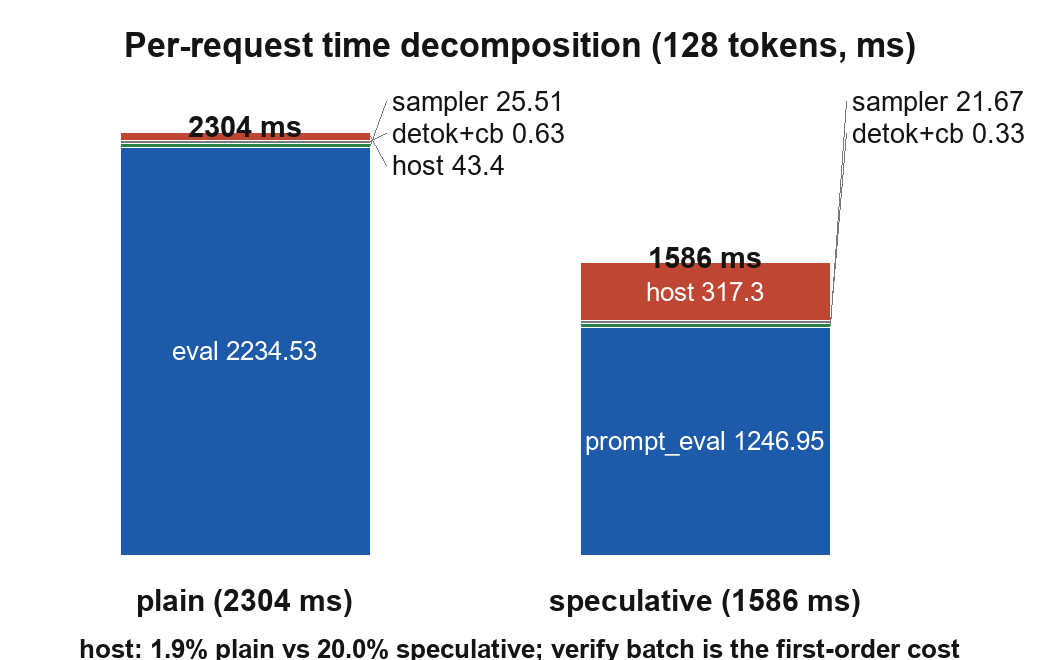
\includegraphics[width=0.98\columnwidth]{fig_attr.png}
\caption{Time decomposition of the same run, plain vs speculative. The
speculative host segment is visible; the multi-row verify batch is the
first-order cost. Under the old subtraction rule the verify block was
misread as host time (91\%).}
\label{fig:attr}
\end{figure}

\section{Capacity Frontier: The 20-Model Matrix}

A single model can be measured well and still mislead, because its walls may be
its own. The matrix asks the same protocol of twenty models, so that the
boundary between what fits and what pages is read from the model set rather
than from one example.

Twenty local GGUF (GPT-Generated Unified Format) models entered one protocol:
16k context, q4 KV, 128 generated tokens, one warmup plus three timed runs.
TTFT was sampled at three prompt tiers with explicit batch 512; rate and
energy followed the engine-default batch.\footnote{Tier token counts read
back from JSON: mostly 317--329 / 2207--2291 / 8507--8831. Default batch is
512 for whitelisted dense architectures, 2 for nextn models, 1 for unknown;
energy sampled at 200\,ms.} Eighteen ran end to end; the full table is
Appendix~\ref{app:matrix} and the capacity--rate picture is plotted in
Figure~\ref{fig:frontier}.

\begin{figure*}[t]
\centering
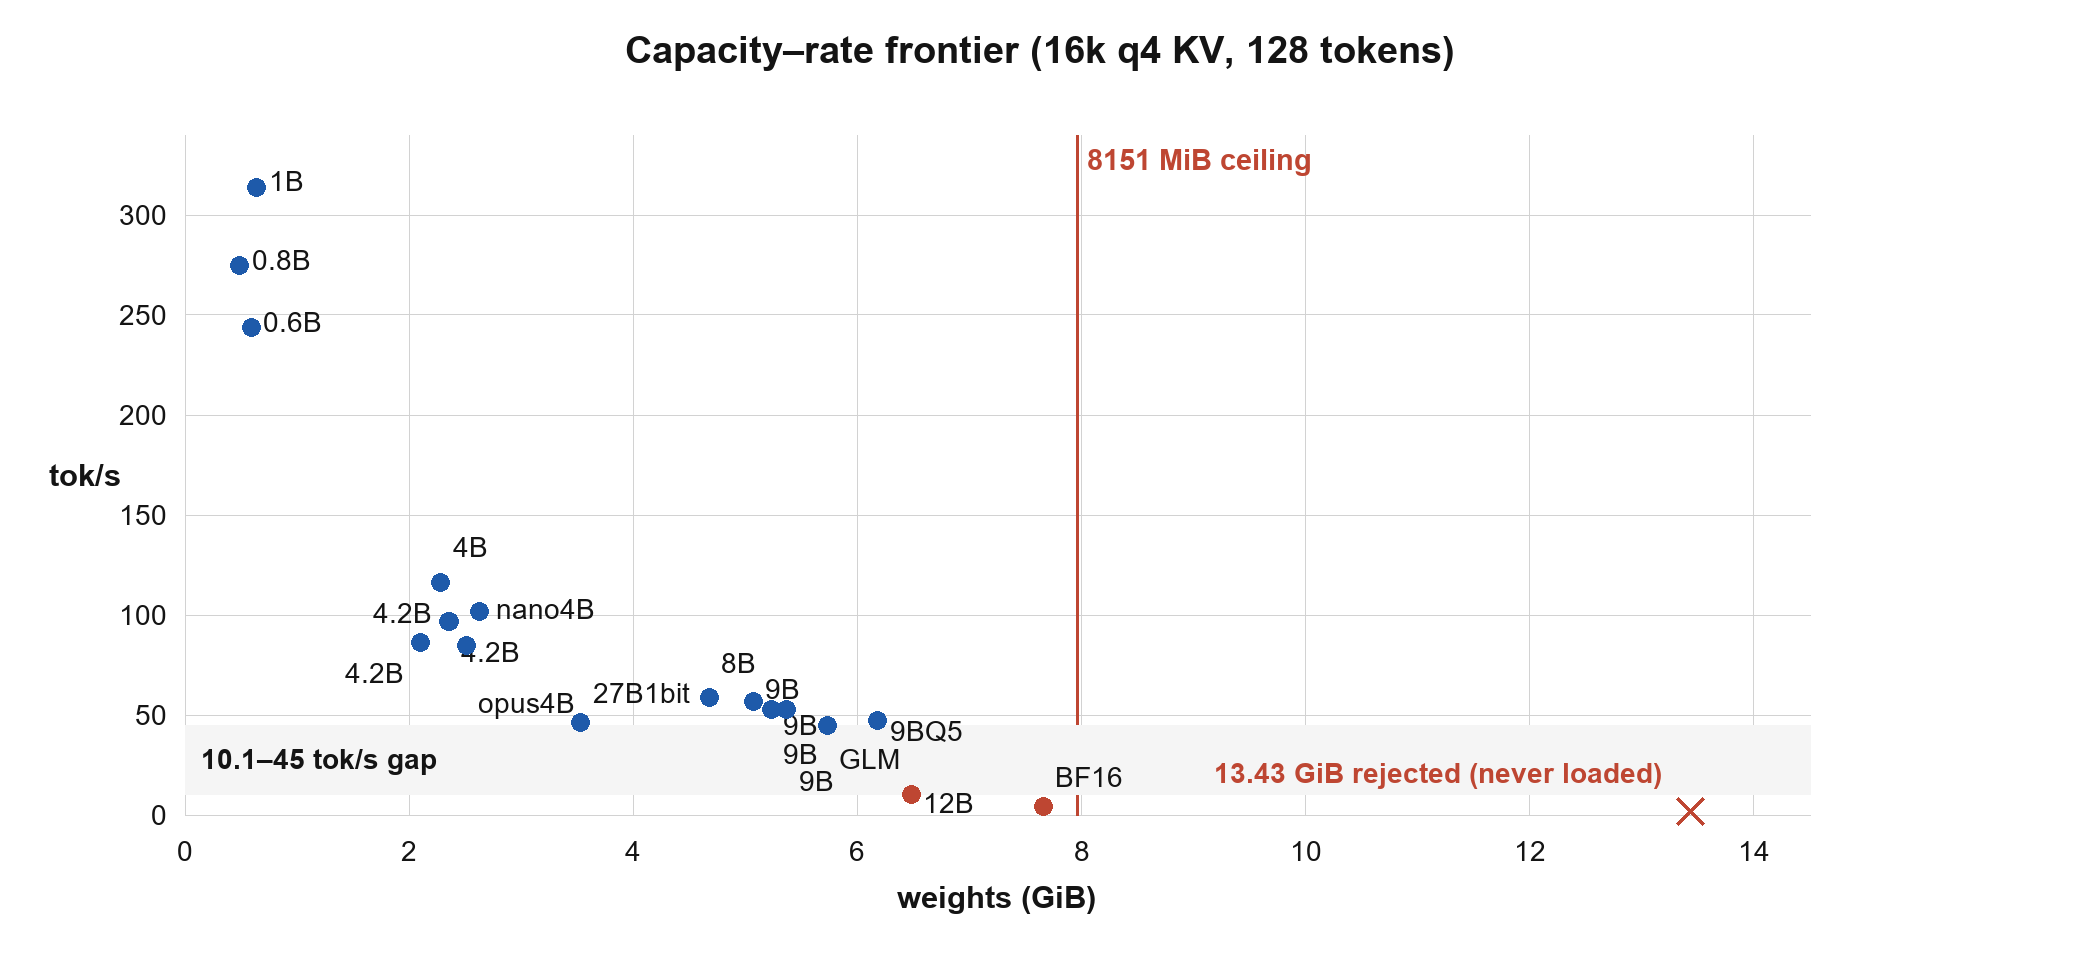
\includegraphics[width=0.92\textwidth]{fig_frontier.png}
\caption{Capacity--rate frontier from the matrix record. The vertical line is
the 8151\,MiB usable ceiling (7.96\,GiB); the 13.43\,GiB model is plotted as
rejected (never loaded). The 10.1--45.0\,tok/s gap separates usable from
paging-bound models; the 1-bit 27\,B sits with the 9\,B class.}
\label{fig:frontier}
\end{figure*}

\textbf{Capacity creates the discontinuity.} Four blocks emerge: nine models
under 3\,GiB with 3.8--6.1\,GiB of headroom; eight at 4.7--6.5\,GiB whose
headroom tightens from 1672 to 435\,MiB; a 7.66\,GiB BF16 model at 470\,MiB;
and a MoE (mixture-of-experts) model with 13.43\,GiB of tensor weights (13{,}755\,MiB, 69\% over
the card; its full GGUF file measures 13.45\,GiB) rejected
pre-load---only metadata parse and budget arithmetic ran. The blocks are not
arbitrary cutoffs; they follow the arithmetic of weights plus KV plus compute
buffers, which is why headroom, not weight size alone, orders the rows.
Footprint tracks layer count and compute buffers: the 1-bit 27\,B
model (3.53\,GiB) peaks above the 4\,B class, and the 12\,B model's weights
exceed the 9\,B Q4\_K\_M's by only 20\% yet its peak is 787\,MiB higher. Rate
tiers are stable (1\,B about 314; 4\,B 85--116; 8\,B 59; 9\,B 47--57 plain,
76--77 speculative; 27\,B 1-bit 46.1), with an empty gap between 10.1 and
45.0\,tok/s: the usable/unusable boundary sits in that 4.5$\times$ void.
Nothing in the matrix lands inside the gap, which is what makes it a boundary
rather than a slope.

\textbf{TTFT is linear in prompt length up to 16k.} Token counts span about
27$\times$ across tiers; TTFT spans 24--29$\times$; no quadratic knee appears.
Linearity is what makes the three-tier protocol adequate: two points predict
the third, and a knee would have shown as a break between tiers.
Per-token slopes track weight bytes (1\,B 0.07--0.08\,ms; 4\,B 0.25; 8\,B
0.48; 9\,B 0.39--0.45; 27\,B 1.24---the last multiplied by 64 layers of fixed
cost). Healthy long-tier TTFT is seconds (9\,B about 3.8\,s, 4\,B about
2.2\,s).

\textbf{Edge degradation: the long-context numbers would measure paging.} The
12\,B model's arithmetic collapses: 6636\,MiB weights + 144\,MiB KV leave
1371\,MiB, but compute buffers, graphs, and CUDA context consume about
937\,MiB more, leaving 435\,MiB---already at the 8-token probe. Its mid-tier
decode runs at 2.199\,tok/s against 10.07 short-tier (22\%); dropping context
16k$\rightarrow$4k recovers only 15\% (11.63) at unchanged peak: weights and
graphs already fill the card. Its long tier and prefill parity are excluded by
the \texttt{vram\_edge} rule. The BF16 model is the same phenomenon one step
worse: the loader places 7843.53\,MiB on device plus 640\,MiB CPU-resident,
and KV (648\,MiB) plus compute (308.55\,MiB) push the total over 8151, so
Windows pages the excess; its 4.2\,tok/s measures swapping. It was stopped
after TTFT (4501.3\,ms at 325 tokens), which together with the peak already
establishes paging.

\textbf{Two parity failures, neither a broken model.} The GLM-4.6V model's
regular 5/130/520-token parity passes; the failure is
\texttt{FAIL(policy\_mismatch)}: the harness expects default batch 512 for
every model, while the engine's whitelist excludes \texttt{glm4} and falls
back to narrow batch---a policy divergence between engine and test; other
non-whitelisted architectures fall back to narrow batch as well. The 0.8\,B
hybrid model fails cross-shape parity at all three tiers (512-row batch vs
token-by-token) while within-batch determinism and default-vs-explicit match
are OK: the same batch-width numerics as Section 4, amplified into sequence
divergence at small scale. Single-mode use is self-consistent, and the model's
rate/TTFT/energy/VRAM were all measured in that mode.

\textbf{Selection-level retreats.} No production default changed during the
matrix. The two retreats were selection-level: 9\,B candidate
Q5\_K\_M$\rightarrow$Q4\_K\_M (headroom doubled, plain faster, acceptance
lower, speculative absolute nearly unchanged), and the 12\,B
16k$\rightarrow$4k diagnostic above. The 4k control also shows KV is not a
major cost for healthy models (0.6\,B gains 243.6$\rightarrow$275.3 because
its 448\,MiB KV is large relative to 0.59\,GiB weights; GLM +5.8\%; others
within $\pm2\%$). The best row is 9\,B Q4\_K\_M: rate, TTFT, and 1222\,MiB
headroom all at the sweet spot. The matrix's answer is a usable envelope:
8151\,MiB buys a 9\,B dense model + 16k q4 KV + width-1 speculation at
6605--7561\,MiB peak; above that, 12\,B pages and 13.43\,GiB never loads.
Whether the engines that run inside that envelope differ at all is the
question of the next section.

\section{Same-Machine Comparison with Upstream and Discernibility Grading}
\label{sec:upstream}

The comparison round fixes everything the matrix varied: same machine, same
GGUF files, same quantization, 16k q4 KV, 128 generated tokens, greedy, seed
1234, the matrix's 6-token prompt. Upstream is the local prebuilt
\texttt{llama-b12202} (commit \texttt{d6be06557}, Clang 20); the fork is the
MSVC + CUDA 13.5 build at \texttt{727fa5c}. Engines are measured in pairs back
to back, order alternated per round; each engine runs one warmup plus three
timed runs, medians reported; power, temperature, and memory clock are logged
throughout. The round is paired for a reason: an engine comparison on a laptop
is dominated by machine state, and pairing removes the state that both engines
share. Grading rule, fixed in advance: cross-round delta spread
$\le$10 percentage points = distinguishable; 10--25 = loose; $>$25 =
unmeasurable, and no directional claim is written for unmeasurable rows
(Table~\ref{tab:upstream}); the full per-model record is
Appendix~\ref{app:abfull} (Table~\ref{tab:upstreamfull}).
Table~\ref{tab:rounds} fixes the conditions of the
three measurement rounds used in this paper; the abstract, introduction, and
conclusion quote only the 520-token round.

\begin{table*}[t]
\centering
\scriptsize
\setlength{\tabcolsep}{4pt}
\begin{tabular}{@{}lllllll@{}}
\toprule
Round & Model / quant & Prompt & Batch widths & Engines & TTFT (ms) & Build \\
\midrule
K1-a (2026-11-11) & 9B Q5\_K\_M & 521-tok agent & MTP 2 / plain 512 & fork vs fork & 9733.55 / 265.28 & 2026-11-11 \\
18-model A/B & 18 models & 6-tok & defaults / 512 & fork vs b12202 & Table~\ref{tab:upstreamfull} & 727fa5c \\
520-token & 9B Q4\_K\_M & 520-tok & 2 / 512 / MTP w1 & fork vs b12202 & Table~\ref{tab:521} & 727fa5c \\
\bottomrule
\end{tabular}
\caption{The three measurement rounds (single source of truth). All rounds:
ctx 16384, q4 KV, greedy, 128 generated tokens, medians of paired repetitions
with alternated engine order. K1-a is a fork-internal contrast on a different
model, quantization, and prompt; it is retained here and in
Figure~\ref{fig:ttft} as the fork-side prefill evolution, not as an upstream
comparison. The 520-token round is the only fork-versus-upstream long-prompt
round quoted in the abstract and conclusion.}
\label{tab:rounds}
\end{table*}

\begin{table}[t]
\centering
\small
\setlength{\tabcolsep}{3pt}
\begin{tabular}{@{}ll>{\raggedright\arraybackslash}p{0.58\columnwidth}@{}}
\toprule
Grade & Models & Result (median $\Delta$; spread) \\
\midrule
dist & 10 & within $\pm1.1\%$; abs.\ mean 0.67\%; 8 higher / 1 lower / 1 tied \\
loose & 1 & $-2.7\%$; 11\,pp \\
unmeas & 7 & no direction claimed; up to 40\% cross-round variation \\
\bottomrule
\end{tabular}
\caption{Grading summary of the same-round 18-model A/B round (plain decode,
6-token prompt). Rule: spread $\le$10\,pp = distinguishable, 10--25 = loose,
$>$25 = unmeasurable. The full per-model record---rates, TTFT, and peak
VRAM---is Appendix~\ref{app:abfull} (Table~\ref{tab:upstreamfull}).}
\label{tab:upstream}
\end{table}

\textbf{Ten models are indistinguishable.} Median deltas all within
$\pm1.1\%$, absolute mean 0.67\%, sign inconsistent (eight higher, one lower,
one tied)---consistent with an earlier same-round isolated retest that landed
within $\pm2\%$ (per-model grading in Appendix~\ref{app:grade}). No stable
difference beyond 2\% appears in the resolvable set.

\textbf{Seven models are unmeasurable.} The same model and engine differ by up
to 40\% across rounds as the envelope switches between 50 and 115\,W; a 1--5\%
engine delta is absorbed. Six of the seven are $\ge$4.68\,GiB; the seventh is
the 2.63\,GiB hybrid with one 29\% outlier---capacity and power at the edge. Their median
deltas reflect power-state noise rather than engine behavior. One further
model is loosely resolved ($-2.7\%$, range $-8$..$+3$\,pp). Resolution requires
locked clocks or stable external power; this round kept system power settings
unchanged.

\textbf{TTFT gaps have a mechanism, and the mechanism is configuration
(Figure~\ref{fig:ttft}).} At 4\,B the fork takes 21.4\,ms against 57.6\,ms, a
2.7-fold gap, because it defaults prefill batch to 512. The 1\,B and 0.8\,B
models move in the same direction. At 9\,B with a nextn head the order
reverses (65.6 vs 61.9\,ms), because the fork defaults that model to batch 2
for numerical alignment. On a 6-token prompt the penalty is small; the
520-token round below measures what it becomes.

\textbf{The 520-token round (Table~\ref{tab:521}, Figure~\ref{fig:521}).} The
18-model round used a 6-token prompt, so a second same-machine round fixes a
520-token prompt (upstream reports \texttt{prompt\_n}=520) and repeats the
paired protocol on the 9\,B Q4\_K\_M model. Decode is indistinguishable:
54.08 against 53.88\,tok/s plain (+0.36\%), 75.20 against 73.21\,tok/s on the
speculative path (+2.7\%). TTFT separates: the fork's default plain path takes
4105\,ms against upstream's 286\,ms, because the nextn model is parity-locked
to batch 2; the fork's explicit-512 path takes 253\,ms, 11\% below upstream's
286\,ms. On the speculative path the fork takes 8280\,ms against upstream's
303\,ms: the fork keeps token-by-token prefill for cross-path parity, while
upstream, which carries no such contract, batches the same MTP prefill. The
27$\times$ gap is the price of the parity contract; closing it is roadmap
item 1. The two paths separate cleanly: decode is where the engines agree, and
prefill is where the contract shows.

\begin{table}[t]
\centering
\small
\setlength{\tabcolsep}{3pt}
\begin{tabular}{@{}lrrrrrr@{}}
\toprule
Path & \multicolumn{2}{c}{tok/s} & \multicolumn{2}{c}{TTFT (ms)} & \multicolumn{2}{c}{Peak (MiB)} \\
\cmidrule(lr){2-3}\cmidrule(lr){4-5}\cmidrule(lr){6-7}
 & fork & upstream & fork & upstream & fork & upstream \\
\midrule
plain default & 54.08 & 53.88 & 4105 & 286 & 6570 & 6178 \\
plain b512 & 54.23 & -- & 253 & -- & 6570 & -- \\
MTP w1 & 75.20 & 73.21 & 8280 & 303 & 6918 & 6551 \\
\bottomrule
\end{tabular}
\caption{520-token same-machine round, 9\,B Q4\_K\_M, 16k q4 KV, greedy,
128 generated tokens; medians of two paired repetitions with alternated
engine order. \texttt{plain b512} is the fork's parity-gated explicit prefill
path; upstream's default batch is already 512, so it has one plain row.}
\label{tab:521}
\end{table}

\begin{figure}[t]
\centering
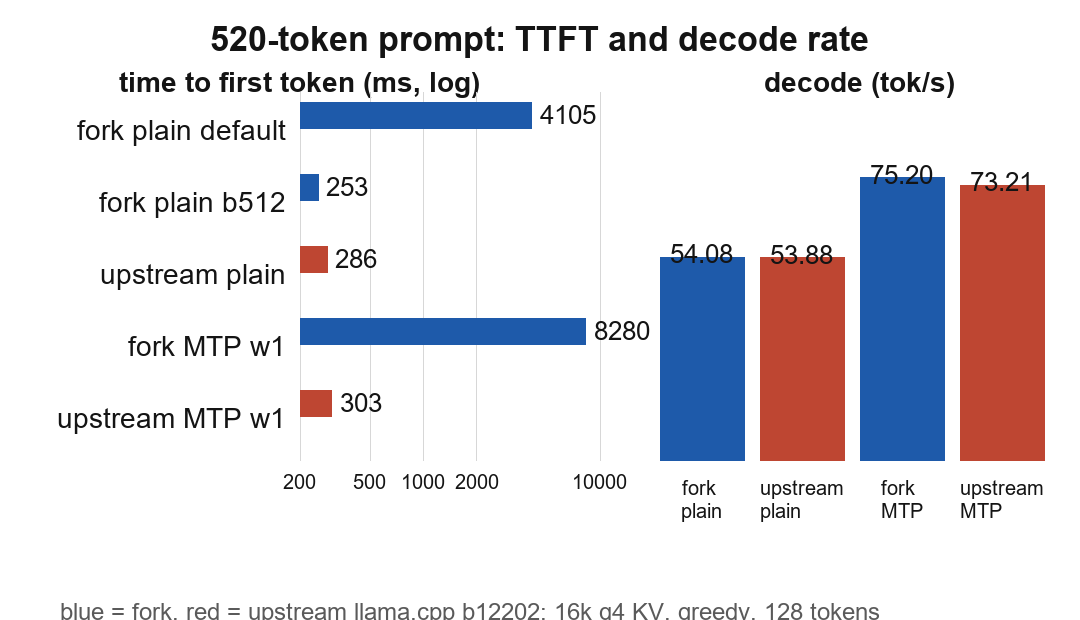
\includegraphics[width=0.98\columnwidth]{fig_521.png}
\caption{The 520-token round: TTFT on a log scale (left) and decode rate
(right). The fork's default prefill is 14$\times$ upstream plain and
27$\times$ upstream speculative, due to its parity-locked default batch width
(2 on this nextn model, against upstream's 512); the explicit-512 path is
11\% below upstream plain's 286\,ms.}
\label{fig:521}
\end{figure}

\begin{figure}[t]
\centering
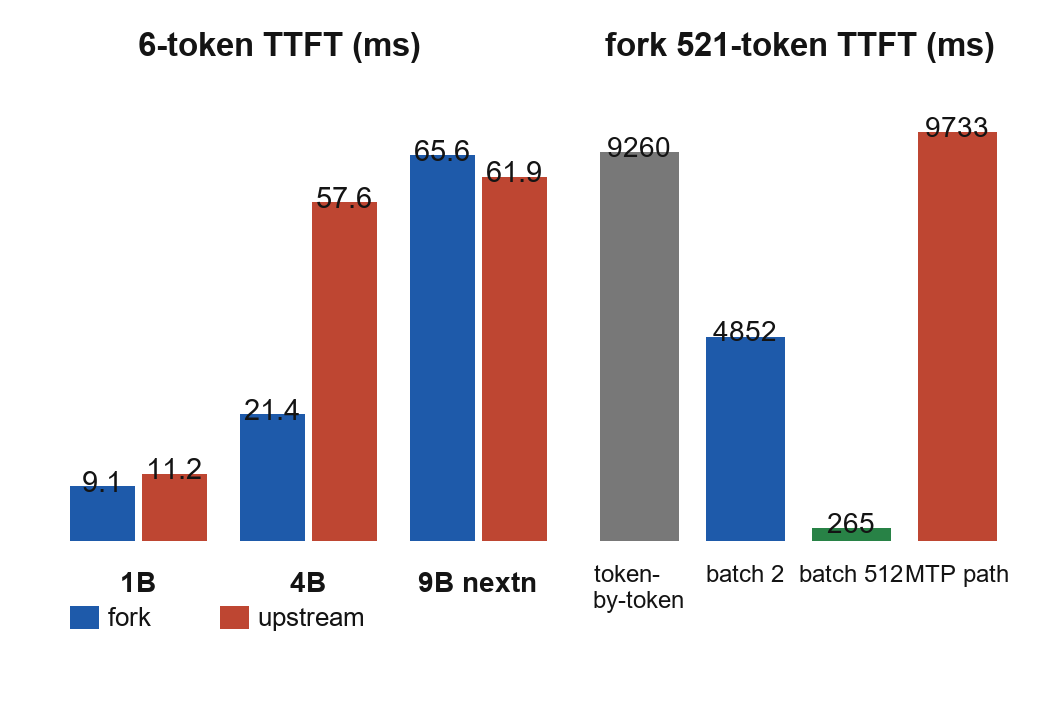
\includegraphics[width=0.98\columnwidth]{fig_ttft.png}
\caption{Left: short-prompt TTFT pairs from the 18-model A/B round---the 4\,B
gap is the fork's default batch 512; the nextn 9\,B reverses because its
default is 2. Right: fork-side 521-token TTFT evolution from the K1-a round
(9B Q5\_K\_M, agent prompt, fork-internal): 9260 token-by-token, 4852 at
batch 2, 265 at batch 512; 9733 on the speculative path.}
\label{fig:ttft}
\end{figure}

\textbf{Peak VRAM averages 6\% higher on the fork across the 18 models.}
4\,B: 5065 vs 4689\,MiB (+8.0\%); 9\,B: 6138 vs 5756\,MiB (+6.6\%)
(Table~\ref{tab:vram}). The excess sits on the
speculative-head and graph-memory side. The original probe (9\,B Q5, 8k q4)
peaked at 7106\,MiB with MTP off and 7607\,MiB with MTP on, leaving 544\,MiB
headroom; its loader-level device split (weights 5491.00, KV 72.00, recurrent
state 50.25, compute 525.29\,MiB; $+$166.49 device
and $+$50.25 state with MTP) plus the desktop baseline reconciles with those
peaks within about 2\%, while the 666.88\,MiB embedding stays CPU-mapped.

\begin{table}[t]
\centering
\small
\setlength{\tabcolsep}{3pt}
\begin{tabular}{@{}lrrl@{}}
\toprule
Model & Fork & Upstream & Condition \\
\midrule
4B Q4\_0 & 5065 & 4689 & 16k q4, 6-tok prompt \\
9B Q4\_0 & 6138 & 5756 & 16k q4, 6-tok prompt \\
\bottomrule
\end{tabular}
\caption{This round's VRAM peaks (MiB), same-round paired conditions.}
\label{tab:vram}
\end{table}

\section{Hardening, and a Taxonomy of Sixteen Measurement Traps}

A read-only audit after the matrix found six gaps, none of them visible as a
runtime crash or a failing test. The first was engine-scoped cancellation: a
cancel in one session could reach another, and the flag was moved to session
scope. The second was a context-length check that compared only against a lower
bound and never against the model's training length. The third was a
zero-training-length pathology that would have rejected every load. The fourth
was an overflow branch that no test had executed. The fifth was a member that
was declared but never read. The sixth was a stats race under concurrent
generation, deliberately left as a documented contract because changing the
snapshot's scope would break the frozen ABI (Appendix~\ref{app:abi}). Each fix
turned its guard red and then green, and the post-hardening gates read
speculative
71.86/71.77/71.08, plain 47.00/47.27/46.80\,tok/s across three runs, parity
64/64. The hybrid Nemotron emits an end-of-generation token at the first step on
the default short prompt (0 generated) but 128 on a long prompt; the round
touches no token-selection code, consistent with model--prompt interaction, and
the matrix pins a period-free prompt.

The project's pitfall log holds sixteen entries in six causal groups
(Appendix~\ref{app:pits}); the groups themselves are the result:
(1)~process-boundary traps (three same-named DLL sets on PATH produce ``loads
fine, first decode illegal access''; negative exit codes defeat
\texttt{if errorlevel 1}; GBK consoles mangle UTF-8 evidence);
(2)~ledgers that pass while wrong (unsynchronized timing leaks 1.73\% into the
next call; the 91\% reversal);
(3)~batch-width numerics (short-prompt flips, token-38 width-2 divergence, and
the env-swallowed false positive);
(4)~speculative state (the last-token trap; rollback slots misused as a
performance knob);
(5)~duplicated policy (engine whitelist vs test expectation; the
unknown-architecture fallback; cancel scope; the Nemotron EOG behavior);
(6)~measurement design (8-token runs reporting 119\,tok/s where 128-token
retests give 95--97; seven models run serially all 5--10\% ``slow'' until
isolated same-round retests land within $\pm2\%$).
Two entries produce no error code, so exit status alone cannot certify them.
The next section turns from the engine's own guards to the systems whose
mechanisms it borrowed.

\section{Prior Systems: Mechanisms Borrowed, Preconditions Failed}

Nine third-party projects were surveyed---the direct upstream plus eight
local snapshots (no \texttt{.git}; identity from \texttt{repos.json} and
download-time metadata). Three are read in detail below: the direct upstream,
Strata, and FlexLLMGen. The remaining systems are each given a short paragraph
of their own (the AirLLM entry covers two relatives), and Table~\ref{tab:oss}
carries every mechanism with its source. Each system is read with three
questions: what
mechanism does it prove, why do its preconditions fail here, and what was taken.
Borrowings are scheduling shapes; the snapshots are engineering systems, not
peer-reviewed papers, and each is cited by its repository identifier.

\textbf{Academic lineage: speculation.} Speculative decoding trades extra
draft work for fewer target reads~\cite{leviathan2023,chen2023spec};
multi-head variants remove the separate draft model~\cite{medusa2024}, and the
native MTP head is the same draft-verify loop inside the
target~\cite{deepseekv3,llamacppmtp}. The measurements below establish the
width-dependent parity boundary and the prefill cost of that loop.

\textbf{Academic lineage: prefill, memory, and measurement.} Sarathi-Serve
introduces chunked prefill and stall-free batching~\cite{sarathi2024};
single-GPU offloading and Flash-based streaming trade bandwidth for
capacity~\cite{flexgen2023,llmflash2024}, and neuron sparsity reduces bytes per
token~\cite{powerinfer2024}. Roofline analysis~\cite{williams2009}, KV
quantization~\cite{kivi2024}, and prefix reuse~\cite{promptcache2024} supply
the measurement and caching vocabulary. What the record adds is a measured
boundary, not a new mechanism.

\textbf{Disk streaming (the direct upstream).} Proves a llama fork can become
a pager without rewriting kernels, at throughput $\approx$ disk bandwidth:
6\,GB per token at 5.56\,GB/s is 1.1\,s/token; Flash-based streaming makes the
same trade~\cite{llmflash2024}. Preconditions fail by an order
of magnitude against a tens-of-ms interactive target; taken: the node-loop
hook point, and disk as a capacity layer only. In this design the hook point
is where the fork's tier-memory slot allocator attaches, and the resident
build disables the hook before the first load (Section~2).

\textbf{Strata (prefix checkpoints, per-width draft policy).}~\cite{Strata2026}
It reports a 262K-token document cold read of 904\,s falling to 0.53\,s median
TTFT for follow-up questions on a P100 when turn boundaries are present, via
verbatim state copies. Its DraftPolicy makes ``speculation is sometimes
negative'' online-decidable, with per-width cost tables and exploration probes.
Preconditions fail: 33--44\,GB RAM model packs against 15.7\,GiB here, no
AVX-512. Taken: prefix checkpointing as evidence input for the probe in
Section 4, and per-width gating as the design response to ngram's $-3\%$. Its
Windows pitfall list became the telemetry field list: WDDM (Windows Display
Driver Model) free-VRAM overstatement, sysmem fallback collapsing
to one-seventh at zero headroom, commit-charge accounting, and a 640\,MiB pin
reserve. In this design the checkpoint shape carries the state-reuse
assumption of the two-round prefix probe (Section~4), the per-width gate
becomes the admission rule that keeps width 2 behind its own 64-token gate
(Section~6), and the pitfall list is the field set the telemetry prints
(Section~7).

\textbf{FlexLLMGen (FlexGen re-distribution)}~\cite{flexgen2023,flexllmgen}. The cost formulas
$T_{gen}=ctog+\max(gtoc,dtoc,ctod,comp)$ and
$T_{pre}=\max(ctog+dtoc,gtoc+ctod,comp)$---decode's weight upload is a serial,
unhideable term; prefill I/O can overlap compute. Taken: the serial/parallel
judgment and amortizing weight reads over MTP's K candidates as an internal
batch; dropped: static percent scheduling and 4$\times$1\,GB pinned relays (a
quarter of this machine's RAM). In this design the serial/parallel split
separates decode's unhideable weight upload from prefill's overlappable I/O in
the ledger (Section~7), and the amortization is why MTP's K candidates are
verified as one batch.

\textbf{KTransformers.}~\cite{ktransformers} It supplies the pinned odd/even
double buffering and the one-behind submission taken here, which are what let
the host path keep a transfer in flight while the previous one retires. Its
preconditions fail on this machine: CMake stops at libnuma, and the AMX/AVX-512
stack it is built around is unusable on this consumer CPU. The borrowed shape
therefore lands as a buffering pattern in the host submission path
(Section~2), without the NUMA and matrix extensions that come with it.

\textbf{Swiftlet.}~\cite{swiftlet} It supplies fixed-stride expert packs and
per-layer LFU slot pools, both of which assume a routed expert model and a
Swift/Metal runtime. Neither holds here: Swift/Metal does not build on this
machine, and no routed-expert model is in the whitelist. The borrowed shapes
survive as design notes for a future expert-streaming line, and the 4\,MB
random-read figure in Section~3 is the side evidence for block sizing.

\textbf{AirLLM family.}~\cite{airllm} It contributes the verbatim
packed-transfer rule and the super-block \texttt{block\_NNN.bin}+index layout.
Its per-layer \texttt{gc+empty\_cache} is a Windows no-op, so the family's own
caching does not transfer; a downstream fork supplies the negative pin evidence
(about 0.7\,GB/s, bf16 and 4-bit)~\cite{rabbitllm}, and one relative's numbers
were rejected outright---its ``compute'' is \texttt{sleep(30\,ms)} and its GPU
cache raises NotImplementedError~\cite{airllmplus}. What lands here is the
layout note for the disk capacity layer, together with the negative sample that
turns hot-path pinning into a measured wall (Section~3).

\textbf{PowerInfer.}~\cite{powerinfer2024,powerinfer} It reduces bytes per token
by exploiting ReLU zeros, a precondition that SwiGLU models do not meet, so the
main mechanism does not apply. Its ExpertCache shape (aligned preallocation,
fixed LRU, deep async reads) survives as a reference component, and its single
Windows datum (2080Ti, 13B Q4, 4.05\,tok/s) sets an order-of-magnitude
reference for what disk-backed serving costs.

Table~\ref{tab:oss} summarizes. The walls are hardware properties; the lever
is bytes per token, layer, and timing---the borrowed scheduling shapes.

\begin{table}[t]
\centering
\small
\setlength{\tabcolsep}{2.6pt}
\hyphenpenalty=10000
\begin{tabular}{@{}>{\raggedright\arraybackslash}p{0.27\columnwidth}>{\raggedright\arraybackslash}p{0.38\columnwidth}>{\raggedright\arraybackslash}p{0.195\columnwidth}@{}}
\toprule
Mechanism (source) & Why preconditions fail here & Disposition \\
\midrule
Disk streaming (upstream) & 5.56\,GB/s vs 6\,GB/token & capacity layer only \\
Tiered residency (FlexGen) & PCIe 26.7\,GB/s; 0.25\,s/token & not used \\
Expert streaming (Swiftlet) & no routed model; Swift/Metal only & design notes \\
Prefix checkpoint (Strata) & RAM packs 33--44\,GB & probe evidence \\
Per-width draft gate (Strata) & --- & adopted shape \\
Pinned double buffer (KTransformers) & NUMA/AMX absent & adopted shape \\
Neuron sparsity (PowerInfer) & SwiGLU, no zero activations & not done \\
Super-block layout (AirLLM family) & disk-bound per layer; cache a no-op & layout note \\
External draft (this work) & draft forward $\ge$ target step & rejected (measured) \\
\bottomrule
\end{tabular}
\caption{Surveyed mechanisms: proven benefit, failed precondition, and
disposition. Nine projects: the direct upstream plus eight snapshots.}
\label{tab:oss}
\end{table}

\section{Threats to Validity, Reproducibility, Data Availability}

The record in Sections~3--10 holds under the conditions listed here.

\textbf{Threats.} One machine, one Windows installation, one local volume; the
fork is frozen at llama.cpp 0.7.0 / ggml 0.27.0, so conclusions hold for that
build, this model set, these quantizations. Upstream is Clang-built, the fork
MSVC + CUDA 13.5: compiler differs between the two engines. The A/B evidence
covers plain decode at a 6-token prompt on 18 models and a 520-token round on
one model;
the prefix probe covers two rounds on
one model's plain path; the cancel-scope guard test passes under the supported
single-threaded contract, which admits no concurrent red case. Cross-round
numbers are trends: the same code differs 8\% between 12001 and 11001\,MHz
memory-clock states. Weight figures use GiB = 1{,}073{,}741{,}824\,B
throughout and quote tensor weights: the rejected model's weights are
13.43\,GiB (14{,}423{,}538{,}808\,B) while its full GGUF file is 13.45\,GiB
(14{,}439{,}363{,}264\,B); the two source numbers measure different quantities
(Appendix~\ref{app:errata}).

\textbf{Reproducibility (commands in Appendix~\ref{app:repro}).} Build: MSVC
(VS 18) + Ninja + CMake, portable CUDA 13.5, \texttt{GGML\_CUDA=ON},
\texttt{CMAKE\_CUDA\_ARCHITECTURES=120}, upstream tests/server/curl off, OpenMP
and native off; one entry script, \texttt{BUILD\_OK} meaning compile-only
(load, env, arch, GPU presence, and tests are separate proofs). Release PATH
carries exactly the build bin and the CUDA runtime bin; the upstream
prebuilt's same-named DLLs stay out of it. The disk-streaming switch is set to
0 before first load. Gates: 4 tests + 2 benches; the rate threshold prints a
warning but exits 0---correctness uses exit codes, performance uses numbers
with conditions. Every number in this paper traces to an append-only raw log
or JSON in the artifact; mutation evidence and correction blocks are
preserved.

\textbf{Data availability.} The anonymized matrix (201 records, single DLL hash
\texttt{286cb71b14f0d5ce}), the A/B CSVs (6-token and 520-token rounds) and
grading, the 520-token prompt and its tokenizer metadata, the probe tables, and
the errata accompany the artifact.

\section{Research Agenda and Conclusion}

The agenda is ordered by milliseconds saved per unit of risk. (1)~Close the
speculative path's 520-token TTFT gap (8280\,ms against upstream's 303\,ms):
chunk the target prefill while holding bitwise parity, gated by the
short-prompt 64-token gate plus the long-prompt cross gate; the plain path's
253\,ms explicit-512 result marks the target order. (2)~Ship prefix
reuse: the probe shows 14.88$\times$ with zero divergence; the design includes
the last-token decode, sufficient rollback slots, and session-scope reuse
without ABI change. (3)~Consolidate the thrice-written policy (engine
whitelist, test expectation, implicit nextn/rules) into one metadata-derived
traits struct shared by engine and tests---infrastructure that keeps (1) and
(2) from silently regressing. (4)~Clarify ABI documentation (stats = last
completed request). (5)~The 9\,B 100\,tok/s kernel target
(27.7$\rightarrow$23.7\,ms/step at width 2): 15\% step reduction, or acceptance
0.685$\rightarrow$0.75, or a cheaper 3-row verify.

The frontier is a measurement problem before it is an optimization problem,
and the call to action is threefold. First, publish the walls---usable VRAM,
measured effective bandwidth, and the power envelope---alongside any engine
delta on client hardware, so that a 17\,tok/s nominal artifact and a 40\%
power-state confounder cannot pass as engine effects. Second, grade comparisons
by discernibility under power-state variance before claiming a direction;
``unmeasurable'' is a result, not a missing number. Third, gate speculative and
chunked-prefill admission on bitwise parity at the width where the benefit is
claimed, and report the prefill cost of that gate rather than folding it into a
decode rate. The artifact ships the probe, the gates, and the round conditions
of Table~\ref{tab:rounds} so these numbers can be re-measured on other 8\,GiB
clients.

\appendix

\section{Glossary}
\label{app:glossary}

\textbf{nextn head / MTP:} the model's native multi-token prediction head; one
mechanism, two names. \textbf{plain / MTP path:} token-by-token decode vs
speculative decode; their greedy outputs are bitwise identical at admitted
configurations. \textbf{acceptance / mean\_len:} fraction of drafted tokens
accepted / tokens produced per verify step. \textbf{Indistinguishable:}
resolvable under the protocol with a delta inside the noise band.
\textbf{Unmeasurable:} the protocol cannot resolve a direction.
\textbf{Pure residency:} all weights in device memory during decode.
\textbf{margin:} top1--top2 logit gap at a greedy step. \textbf{parity:}
bitwise identical token sequences across paths or configurations, stated with
width and batch. \textbf{n\_rs\_seq:} recurrent-state rollback slots for
hybrid models. \textbf{roofline:} weight bytes $\times$ rate folded to GB/s,
compared against the measured 330\,GB/s interval, per path (MTP amortizes by
mean\_len).

\section{Frozen C ABI Details}
\label{app:abi}

The ABI was frozen at 11 functions and 6 structs, later appended to 14 and 8
without a version bump. Input structs reject undersized callers; output structs
accept size 0 (header-only query), truncate to the caller's size, and backfill
the library's true size---append-only growth is safe for old hosts, and
truncated fields hold caller memory values unless zeroed. Eight error codes
separate cancellation (session reusable) from model/OOM errors (session
undefined); an atomic cancel flag, moved from engine to session scope during
hardening, is the only cross-thread write. There are no locks: one engine serves
one generation at a time, and the stats snapshot is engine-scoped, documented as
``last completed request.'' These rules fix what a measurement may assume:
single-stream generation, a reusable cancelled session, and a stats snapshot
that always describes the previous request.

\section{Full 20-Model Matrix}
\label{app:matrix}

This appendix gives the full 20-model matrix referenced in Section~8, under
one protocol: 16k context, q4 KV, 128 generated tokens, one warmup plus three
timed runs.

\begin{table*}[t]
\centering
\scriptsize
\setlength{\tabcolsep}{3pt}
\begin{tabular}{@{}lrrrrrl@{}}
\toprule
Model & GiB & plain tok/s & MTP tok/s (acc) & TTFT S/M/L (ms) & Peak MiB & Status \\
\midrule
minicpm5-1b & 0.64 & 313.9 & -- & 23.3 / 142.7 / 685.0 & 1898 & measured \\
qwen35-0.8b-q4km & 0.49 & 274.6 & -- & 25.4 / 148.2 / 585.1 & 2032 & cross-shape parity fail \\
qwen3-0.6b-q8 & 0.59 & 243.6 & -- & 20.8 / 131.3 / 692.8 & 2366 & measured \\
nemotron-4b-q4\_0 & 2.28 & 116.1 & -- & 83.7 / 522.1 / 2194.2 & 3634 & measured \\
nemotron-nano-4b-q4km & 2.63 & 101.8 & -- & 90.0 / 553.9 / 2271.5 & 3962 & measured \\
qwen35-4.2b-iq4xs & 2.35 & 97.0 & -- & 88.1 / 543.9 / 2201.3 & 4064 & measured \\
qwen35-4.2b-q4\_0 & 2.36 & 96.7 & -- & 85.0 / 528.9 / 2152.9 & 4084 & measured \\
qwen35-4.2b-q3km & 2.10 & 86.2 & -- & 101.0 / 639.5 / 2564.9 & 3830 & measured \\
qwen35-opus-4b & 2.51 & 84.9 & -- & 96.2 / 593.1 / 2360.6 & 4247 & measured \\
dsr1-8b-q4km & 4.68 & 59.0 & -- & 153.0 / 951.4 / 4147.2 & 6479 & measured \\
qwen9b-q4\_0 & 5.07 & 56.8 & 77.3 (0.767) & 141.1 / 858.7 / 3401.7 & 6605 & measured, w1 parity 64/64 \\
q3.5-9b & 5.23 & 52.9 & -- & 161.6 / 972.2 / 3768.5 & 6581 & measured \\
qwythos9b & 5.23 & 52.7 & -- & 162.6 / 969.8 / 3763.5 & 6581 & measured \\
qwen9b-q4km & 5.37 & 53.0 & 77.2 (0.855) & 162.9 / 968.9 / 3771.7 & 6929 & measured, w1 parity 64/64 \\
qwen9b-q5km & 6.18 & 47.2 & 75.8 (1.000) & 169.0 / 1001.5 / 3878.0 & 7561 & measured, w1 parity 64/64 \\
bonsai-27b-q1\_0 & 3.53 & 46.1 & -- & 424.0 / 2720.3 / 10723.9 & 5396 & measured \\
glm4.6v-q4km & 5.73 & 45.0 & -- & 167.2 / 1051.3 / 4515.1 & 7137 & policy mismatch \\
gemma4-12b-q4\_0 & 6.48 & 10.1 & -- & 5214.0 / 49089.4 / skipped & 7716 & edge degradation \\
spark-x2.5-4b & 7.66 & 4.2 & -- & 4501.3 / stopped / stopped & 7681 & user stop (paging) \\
gemma4-26b-a4b & 13.43 & -- & -- & -- & -- & rejected pre-load \\
\bottomrule
\end{tabular}
\caption{Full matrix, 16k q4 KV, 128 generated tokens, one warmup + three
timed runs. Rate uses engine-default batch; TTFT columns use explicit batch
512. Skips carry reasons (\texttt{vram\_edge}, user stop). MTP rows are width
1; width-2 results appear in Section 6.}
\label{tab:matrix}
\end{table*}

\section{Discernibility Grading of the A/B Round}
\label{app:grade}

This appendix gives the per-model grading behind Table~\ref{tab:upstream} and
the counts in Section~9, under the rule fixed before the round: spread
$\le$10\,pp distinguishable, 10--25 loose, $>$25 unmeasurable.

\begin{table}[t]
\centering
\footnotesize
\setlength{\tabcolsep}{3pt}
\begin{tabular}{@{}lrrl@{}}
\toprule
Model & $\Delta$ med & Spread (pp) & Grade \\
\midrule
minicpm5-1b & +0.5\% & 2 & distinguishable \\
qwen35-0.8b & $-$0.9\% & 2 & distinguishable \\
qwen3-0.6b & +0.9\% & 6 & distinguishable \\
nemotron-4b & +0.9\% & 0 & distinguishable \\
qwen35-4.2b-iq4xs & +0.1\% & 1 & distinguishable \\
qwen35-4.2b-q4\_0 & +1.1\% & 6 & distinguishable \\
qwen35-4.2b-q3km & $-$0.0\% & 1 & distinguishable \\
qwen35-opus-4b & +0.8\% & 2 & distinguishable \\
qwen9b-q4\_0 & +0.5\% & 1 & distinguishable \\
qwythos9b & +1.0\% & 6 & distinguishable \\
bonsai-27b & $-$2.7\% & 11 & loose \\
nemotron-nano-4b & $-$0.8\% & 30 & unmeasurable \\
dsr1-8b & +4.6\% & 42 & unmeasurable \\
q3.5-9b & +0.6\% & 76 & unmeasurable \\
qwen9b-q4km & +1.8\% & 50 & unmeasurable \\
glm4.6v & $-$14.9\% & 60 & unmeasurable \\
qwen9b-q5km & +1.1\% & 71 & unmeasurable \\
gemma4-12b & +13.2\% & 81 & unmeasurable \\
\bottomrule
\end{tabular}
\caption{Grading of all 18 tested models: 10 distinguishable, 7 unmeasurable,
1 loose. The single loosely resolved model is bonsai-27b-q1\_0 (spread 11\,pp);
the 29\% outlier (nemotron-nano, spread 30\,pp) is inside the unmeasurable
group, not the loose one. Spread = max$-$min of valid paired deltas across
rounds, in percentage points.}
\label{tab:grade}
\end{table}

\section{Sixteen Pitfalls in Six Causal Groups}
\label{app:pits}

This appendix gives the sixteen-entry pitfall log summarized in Section~10,
grouped by cause rather than by symptom.

\begin{table*}[t]
\centering
\scriptsize
\setlength{\tabcolsep}{3pt}
\begin{tabular}{@{}clp{0.30\textwidth}p{0.34\textwidth}@{}}
\toprule
\# & Group & Phenomenon & Root cause / resolution \\
\midrule
1 & boundary & loads OK, first decode CUDA illegal access & three same-named DLL sets on PATH; narrow PATH, fixed order \\
2 & boundary & crash \texttt{0xC0000005} treated as pass & \texttt{if errorlevel 1} blind to negative codes; add \texttt{if not errorlevel 0} \\
3 & boundary & CJK evidence mangled, parsers miss keys & GBK console; write UTF-8 files, console ASCII only \\
4 & ledger & decode vs step wall-clock differ 1.73\% & unsynchronized timing leaks into next call; sync+reset after prefill \\
5 & ledger & host computed at 91\% & verify batch books in prompt\_eval; missing term + leak; 1.9\%/20.0\% after fix \\
6 & numerics & short prompt flips at wide batch, long stable & kernel switch + 0.13 chunked shift vs 0.0549/0.0080 margins; cross gate at long tier \\
7 & numerics & Q4\_0 w2 diverges at token 38, rate looks fine & quantization $\times$ width near-tie; parity before rate, width stated \\
8 & numerics & wide-batch log bitwise identical to narrow & env never entered process; require in-band witness, keep CORRECTION block \\
9 & state & prefix continuation mostly wrong after first tokens & last sampled token never decoded; decode final row before reuse \\
10 & state & draft-context slots drop w2 84.2$\rightarrow$80.3 & rollback slots serve correctness; reverted \\
11 & policy & unknown arch 30$\times$ slow, tests green & whitelist fallback 1; shared traits struct proposed \\
12 & policy & default 2$\rightarrow$1 mutation stays green & test expects from meta, engine from whitelist; nearest-neighbor criterion + shared traits \\
13 & policy & cancel A stops B & flag at engine scope; moved to session (7 sites), guard test \\
14 & policy & Nemotron generates 0 on short prompt & sentence-final EOG interaction; pin period-free prompt \\
15 & design & 8-token run reports 119 tok/s & favorable cache/clock window; 128-token retest 95--97; short runs prove liveness only \\
16 & design & serial 7-model sweep all 5--10\% slow & heat/power drift, no same-round baseline; isolated retest within $\pm2\%$ \\
\bottomrule
\end{tabular}
\caption{The pitfall log, grouped by cause. Entries \#5 and \#12 produce no
error code. Entries preserve their original correction blocks in the
artifact.}
\label{tab:pits}
\end{table*}

\section{Reproduction Commands}
\label{app:repro}

Build with the single entry script (vcvars64, then portable CUDA 13.5 on PATH,
then CMake+Ninja; arch 120; upstream tests/server/curl off). Run the P0 gate
(4 tests + 2 benches; rate threshold advisory, exit codes authoritative). Run
the matrix driver with the model registry (\texttt{--dry-run} first;
\texttt{--run-id full1}); per-model pilot via \texttt{--models}. Run the A/B
repeats with two rounds and alternating engine order, then the stability
fix-pass that validates power ($\ge$80\,W) and memory-clock ($\le$500\,MHz
difference) before accepting a pair. Verify the 64-token parity gate before
any width or batch change. Energy via the 200\,ms polling script; margins via
the env-gated oracle. Checksums, the anonymous model registry, raw logs, and
correction blocks accompany the artifact.

\section{Errata Summary}
\label{app:errata}

The source reports contain OCR variants (\texttt{Ilama}, \texttt{11ama}),
invalid table-of-contents page tokens, residual LaTeX arrays, a pageable-PCIe
conflict (3.28 vs 8.28\,GB/s at 512\,MiB; the probe record's 8.28 is adopted),
a missing intermediate TTFT (4852\,ms) in one English abstract, a
project/snapshot count mismatch (9 named projects vs 8 local snapshots),
duplicated abstracts/contents, and the 13.43 vs 13.45\,GiB pair for the
rejected model, resolved as tensor weights (14{,}423{,}538{,}808\,B) vs full
GGUF file size (14{,}439{,}363{,}264\,B) read from the same matrix record.
Author identity present in one source PDF/DOCX
is excluded from this submission. The 91\% attribution and the old small-model
host percentages are retained with correction blocks; the latter serve as
relative ordering.

\section{Full 18-Model A/B Record}
\label{app:abfull}

Table~\ref{tab:upstreamfull} lists every model behind the summary in
Section~\ref{sec:upstream}.

\begin{table*}[t]
\centering
\scriptsize
\setlength{\tabcolsep}{3.2pt}
\begin{tabular}{@{}lrrrrlrrrrr@{}}
\toprule
Model & GiB & TIR tok/s & Up tok/s & $\Delta$ med & Range (pp) & Grade & TTFT T & TTFT U & Peak T & Peak U \\
\midrule
minicpm5-1b & 0.64 & 323.11 & 320.18 & +0.5\% & 0..2 & dist & 9.1 & 11.2 & 2942 & 2714 \\
qwen35-0.8b-q4km & 0.49 & 290.50 & 293.09 & $-$0.9\% & $-$1..1 & dist & 11.1 & 23.1 & 3633 & 3224 \\
qwen3-0.6b-q8 & 0.59 & 286.14 & 284.58 & +0.9\% & 0..6 & dist & 13.9 & 12.8 & 2346 & 2124 \\
nemotron-4b-q4\_0 & 2.28 & 111.74 & 110.74 & +0.9\% & 1..1 & dist & 17.8 & 63.4 & 4874 & 4714 \\
nemotron-nano-4b-q4km & 2.63 & 85.03 & 96.80 & $-$0.8\% & $-$29..1 & unmeas & 19.3 & 65.0 & 3780 & 3620 \\
qwen35-4.2b-iq4xs & 2.35 & 93.97 & 94.02 & +0.1\% & 0..1 & dist & 21.9 & 50.8 & 5430 & 5054 \\
qwen35-4.2b-q4\_0 & 2.36 & 93.96 & 91.90 & +1.1\% & 0..6 & dist & 21.4 & 57.6 & 5065 & 4689 \\
qwen35-4.2b-q3km & 2.10 & 86.64 & 86.21 & $-$0.0\% & 0..1 & dist & 27.3 & 60.8 & 5220 & 4844 \\
qwen35-opus-4b & 2.51 & 83.44 & 83.09 & +0.8\% & 0..2 & dist & 23.3 & 59.2 & 4190 & 3814 \\
qwen9b-q4\_0 & 5.07 & 56.65 & 56.64 & +0.5\% & 0..1 & dist & 65.6 & 61.9 & 6138 & 5756 \\
q3.5-9b & 5.23 & 52.45 & 52.25 & +0.6\% & $-$34..42 & unmeas & 46.6 & 84.0 & 6458 & 6074 \\
dsr1-8b-q4km & 4.68 & 58.59 & 49.43 & +4.6\% & 0..42 & unmeas & 43.5 & 32.5 & 6364 & 6144 \\
qwythos9b & 5.23 & 48.91 & 48.67 & +1.0\% & 0..6 & dist & 46.7 & 89.8 & 6458 & 6074 \\
bonsai-27b-q1\_0 & 3.53 & 44.35 & 47.41 & $-$2.7\% & $-$8..3 & loose & 61.7 & 147.4 & 5332 & 4976 \\
glm4.6v-q4km & 5.73 & 41.87 & 46.70 & $-$14.9\% & $-$58..2 & unmeas & 128.9 & 38.1 & 6984 & 6770 \\
qwen9b-q5km & 6.18 & 41.73 & 46.64 & +1.1\% & $-$69..2 & unmeas & 91.5 & 90.6 & 7149 & 6767 \\
qwen9b-q4km & 5.37 & 51.54 & 44.99 & +1.8\% & $-$8..42 & unmeas & 79.4 & 86.0 & 6456 & 6074 \\
gemma4-12b-q4\_0 & 6.48 & 14.91 & 14.05 & +13.2\% & $-$11..70 & unmeas & 441.5 & 386.9 & 7576 & 7584 \\
\bottomrule
\end{tabular}
\caption{Full per-model record behind Table~\ref{tab:upstream}: same-round
paired comparison, 18 models, plain decode at the 6-token prompt (TTFT in ms;
peaks in MiB). ``dist'' = spread $\le$10\,pp; ``loose'' = 10--25; ``unmeas'' =
$>$25, no direction claimed.}
\label{tab:upstreamfull}
\end{table*}

% All 22 entries are cited and verified against primary sources (2026-11-17).
\clearpage
\bibliographystyle{plainurl}
\bibliography{references}

\end{document}